\begin{itemize}
    \item Go to: \url{www.r-project.org}
    \item Select the download R hyperlink:
        \begin{figure}[H]
            \centering
            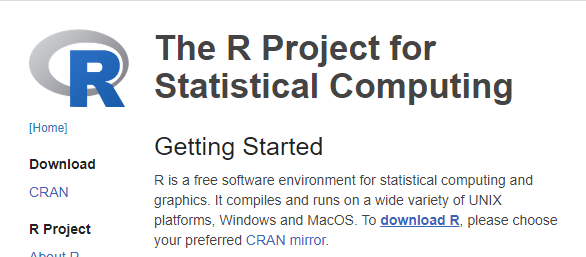
\includegraphics[width=0.4\textwidth]{./Figs/2020-12-25-23-42-12.png}
        % 	\caption{}
        \end{figure}
    
    \item Select the mirors you want, selecting the Cloud options will automatically find the closest server and start downloading from there according to your location.
        \begin{figure}[H]
            \centering
            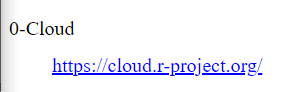
\includegraphics[width=0.4\textwidth]{./Figs/2020-12-25-23-43-12.png}
        % 	\caption{}
        \end{figure}
    
        
    \item Next you will see the comprehensive R archive network and click of your operating system:
        \begin{figure}[H]
            \centering
            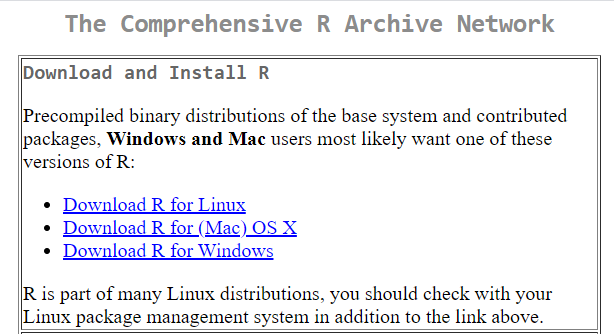
\includegraphics[width=0.4\textwidth]{./Figs/2020-12-25-23-44-20.png}
        % 	\caption{}
        \end{figure}
    
    \item On a Mac click on the latest package file, on windows click base:
        \begin{figure}[H]
            \centering
            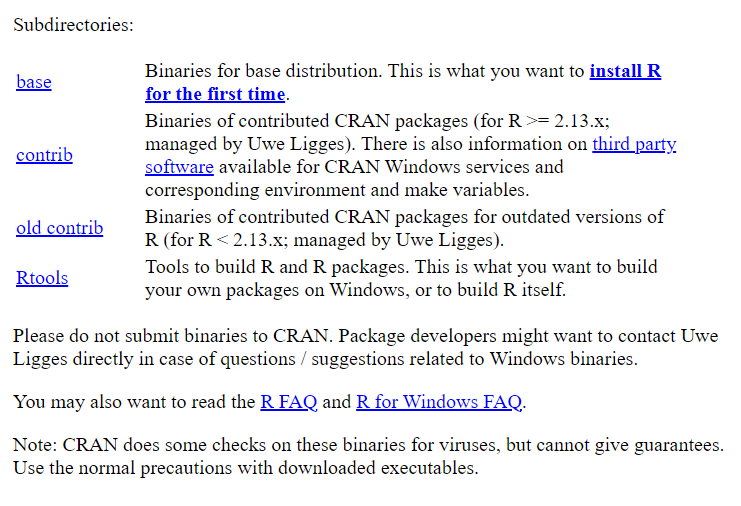
\includegraphics[width=0.4\textwidth]{./Figs/2020-12-25-23-45-06.png}
        % 	\caption{}
        \end{figure}
    
    \item 
\end{itemize}
